% Options for packages loaded elsewhere
\PassOptionsToPackage{unicode}{hyperref}
\PassOptionsToPackage{hyphens}{url}
\documentclass[
  11pt,
  a4paper,
]{article}
\usepackage{xcolor}
\usepackage[margin=22mm,headheight=15pt]{geometry}
\usepackage{amsmath,amssymb}
\setcounter{secnumdepth}{-\maxdimen} % remove section numbering
\usepackage{iftex}
\ifPDFTeX
  \usepackage[T1]{fontenc}
  \usepackage[utf8]{inputenc}
  \usepackage{textcomp} % provide euro and other symbols
\else % if luatex or xetex
  \usepackage{unicode-math} % this also loads fontspec
  \defaultfontfeatures{Scale=MatchLowercase}
  \defaultfontfeatures[\rmfamily]{Ligatures=TeX,Scale=1}
\fi
\usepackage{lmodern}
\ifPDFTeX\else
  % xetex/luatex font selection
\fi
% Use upquote if available, for straight quotes in verbatim environments
\IfFileExists{upquote.sty}{\usepackage{upquote}}{}
\IfFileExists{microtype.sty}{% use microtype if available
  \usepackage[]{microtype}
  \UseMicrotypeSet[protrusion]{basicmath} % disable protrusion for tt fonts
}{}
\makeatletter
\@ifundefined{KOMAClassName}{% if non-KOMA class
  \IfFileExists{parskip.sty}{%
    \usepackage{parskip}
  }{% else
    \setlength{\parindent}{0pt}
    \setlength{\parskip}{6pt plus 2pt minus 1pt}}
}{% if KOMA class
  \KOMAoptions{parskip=half}}
\makeatother
\usepackage{longtable,booktabs,array}
\usepackage{caption}
\captionsetup[table]{skip=6pt}
\newcounter{none} % for unnumbered tables
\usepackage{calc} % for calculating minipage widths
% Correct order of tables after \paragraph or \subparagraph
\usepackage{etoolbox}
\makeatletter
\patchcmd\longtable{\par}{\if@noskipsec\mbox{}\fi\par}{}{}
\makeatother
% Allow footnotes in longtable head/foot
\IfFileExists{footnotehyper.sty}{\usepackage{footnotehyper}}{\usepackage{footnote}}
\makesavenoteenv{longtable}
\usepackage{graphicx}
\makeatletter
\newsavebox\pandoc@box
\newcommand*\pandocbounded[1]{% scales image to fit in text height/width
  \sbox\pandoc@box{#1}%
  \Gscale@div\@tempa{\textheight}{\dimexpr\ht\pandoc@box+\dp\pandoc@box\relax}%
  \Gscale@div\@tempb{\linewidth}{\wd\pandoc@box}%
  \ifdim\@tempb\p@<\@tempa\p@\let\@tempa\@tempb\fi% select the smaller of both
  \ifdim\@tempa\p@<\p@\scalebox{\@tempa}{\usebox\pandoc@box}%
  \else\usebox{\pandoc@box}%
  \fi%
}
% Set default figure placement to htbp
\def\fps@figure{htbp}
\makeatother
\setlength{\emergencystretch}{3em} % prevent overfull lines
\providecommand{\tightlist}{%
  \setlength{\itemsep}{0pt}\setlength{\parskip}{0pt}}
% YOCO notes; style adapted from Attention/CN/pdf-header.tex.
\usepackage{fontspec}
\usepackage{enumitem}
\usepackage{fancyhdr}
\usepackage{fvextra}
\usepackage{etoolbox}
\usepackage{pdflscape}

\setmainfont[
  Path=/usr/local/texlive/2026/texmf-dist/fonts/opentype/public/tex-gyre/,
  UprightFont=texgyrepagella-regular.otf,
  BoldFont=texgyrepagella-bold.otf,
  ItalicFont=texgyrepagella-italic.otf,
  BoldItalicFont=texgyrepagella-bolditalic.otf
]{texgyrepagella-regular.otf}
\setsansfont[
  Path=/usr/local/texlive/2026/texmf-dist/fonts/opentype/public/tex-gyre/,
  UprightFont=texgyreheros-regular.otf,
  BoldFont=texgyreheros-bold.otf,
  ItalicFont=texgyreheros-italic.otf,
  BoldItalicFont=texgyreheros-bolditalic.otf
]{texgyreheros-regular.otf}
\setmonofont[
  Path=/usr/local/texlive/2026/texmf-dist/fonts/opentype/google/roboto/,
  UprightFont=RobotoMono-Regular.otf,
  BoldFont=RobotoMono-Bold.otf,
  ItalicFont=RobotoMono-Italic.otf,
  BoldItalicFont=RobotoMono-BoldItalic.otf,
  Scale=0.82
]{RobotoMono-Regular.otf}
\definecolor{attentionblue}{HTML}{174A7E}
\definecolor{attentiongray}{HTML}{5D6773}
\definecolor{attentionlink}{HTML}{1769AA}
\definecolor{codebg}{HTML}{F4F6F8}

\AtBeginDocument{%
  \hypersetup{
    linkcolor=attentionblue,
    urlcolor=attentionlink,
    citecolor=attentionblue,
    pdftitle={YOCO: Cross-Layer KV Sharing}
  }%
}

\usepackage{titlesec}
\titleformat{\section}
  {\LARGE\bfseries\sffamily\color{attentionblue}}{}{0pt}{}
\titleformat{\subsection}
  {\Large\bfseries\sffamily\color{attentionblue}}{}{0pt}{}
\titleformat{\subsubsection}
  {\large\bfseries\sffamily\color{attentiongray}}{}{0pt}{}
\titlespacing*{\section}{0pt}{1.8ex}{1.2ex}
\titlespacing*{\subsection}{0pt}{1.6ex}{0.9ex}
\titlespacing*{\subsubsection}{0pt}{1.4ex}{0.7ex}

\setlength{\parindent}{2em}
\setlength{\parskip}{0.35em}
\linespread{1.18}
\setlist{itemsep=0.25em,topsep=0.45em,leftmargin=2.4em}
\setcounter{tocdepth}{2}
\setcounter{secnumdepth}{0}

\pagestyle{fancy}
\fancyhf{}
\fancyhead[L]{\small\sffamily\color{attentiongray} YOCO}
\fancyhead[R]{\small\sffamily\color{attentiongray} Purshow’ Notes}
\fancyfoot[C]{\small\sffamily\thepage}
\renewcommand{\headrulewidth}{0.3pt}


\usepackage{caption}
\captionsetup{font=small,labelfont=bf}
\clearcaptionsetup{table} % Overview has no caption; clear Pandoc defaults.
\usepackage{float}
\floatplacement{figure}{H}
\AtBeginDocument{\renewcommand{\figurename}{Figure}}

% A single opening page: article title above an automatically linked contents.
\makeatletter
\renewcommand*\l@subsection{\@dottedtocline{2}{0em}{0em}}
\renewcommand*\l@subsubsection{\@dottedtocline{3}{1.6em}{0em}}
\makeatother
\newcommand{\NotesCover}[1]{%
  \pagenumbering{roman}%
  \thispagestyle{empty}%
  \vspace*{0mm}%
  {\centering
    \sffamily\bfseries\color{attentionblue}%
    \fontsize{26pt}{36pt}\selectfont #1\par
  }%
  \vspace{4mm}%
  {\color{attentionblue}\noindent\rule{\linewidth}{0.6pt}\par}%
  \vspace{4mm}%
  \begingroup
    \setlength{\parindent}{0pt}%
    \setlength{\parskip}{0.6em}%
    \tableofcontents
  \endgroup
}
\newcommand{\NotesCoverEnd}{%
  \clearpage
  \pagenumbering{arabic}%
}

% Compact wrapping overview table, following Attention and MoE notes.
\newcommand{\OverviewTableStyle}{%
  \fontsize{7.5pt}{8.8pt}\selectfont
  \setlength{\tabcolsep}{4pt}%
  \renewcommand{\arraystretch}{1.2}%
  \setlength{\extrarowheight}{6pt}%
  \setlength{\LTpre}{30pt}%
  \setlength{\LTpost}{0pt}%
  \setlength{\parskip}{0pt}%
}
\usepackage{bookmark}
\IfFileExists{xurl.sty}{\usepackage{xurl}}{} % add URL line breaks if available
\urlstyle{same}
% fallback for those not using the hyperref driver hyperxmp:
\makeatletter
\@ifundefined{xmpquote}{\newcommand{\xmpquote}[1]{#1}}{}
\makeatother
\hypersetup{
  hidelinks,
  pdfcreator={LaTeX via pandoc}}

\author{}
\date{}

\begin{document}

\NotesCover{YOCO: Cross-Layer KV Sharing}\NotesCoverEnd

With the release of DeepSeek-V4.1-Flash, YOCO has come back into the
spotlight. In my view, YOCO is an excellent piece of work, and several
interesting variants have emerged from it.

YOCO has two main motivations:

\begin{enumerate}
\def\labelenumi{\arabic{enumi}.}
\item
  \textbf{Prefill--Decode (PD) asymmetry.} The main job of Prefill is to
  build the cache. Only the last prompt token needs to produce the first
  logits; earlier tokens do not need to compute logits at all. A
  standard Transformer struggles to fully exploit this asymmetry because
  each layer needs its own KV Cache. YOCO instead lets the later
  Cross-Decoder layers share a single global Shared KV, allowing earlier
  tokens in a long Prefill to exit as soon as the Shared KV has been
  built. This substantially amplifies the benefits of PD asymmetry. (Su
  Jianlin has also discussed this on Zhihu.)
\item
  \textbf{Compressing the KV Cache along the layer dimension.} KV Cache
  size can be viewed approximately as the product of three dimensions:
  entry (dimensionality and number of heads) × sequence (length) × layer
  (number of layers). Previous work has already compressed it along
  different dimensions:

  \begin{itemize}
  \tightlist
  \item
    \textbf{Entry}: GQA/MQA reduce the number of KV heads, while MLA
    compresses the per-token KV representation dimension
    \(d_{\mathrm{KV}}\).
  \item
    \textbf{Sequence}: Attention mechanisms such as CSA/HCA/Linear
    reduce the caching requirements associated with the history length
    \(N\).
  \item
    \textbf{Layer}: YOCO-style methods target the layer dimension,
    letting later layers share a single global KV Cache.
  \end{itemize}
\end{enumerate}

\subsection{1. YOCO}\label{yoco}

\begin{center}

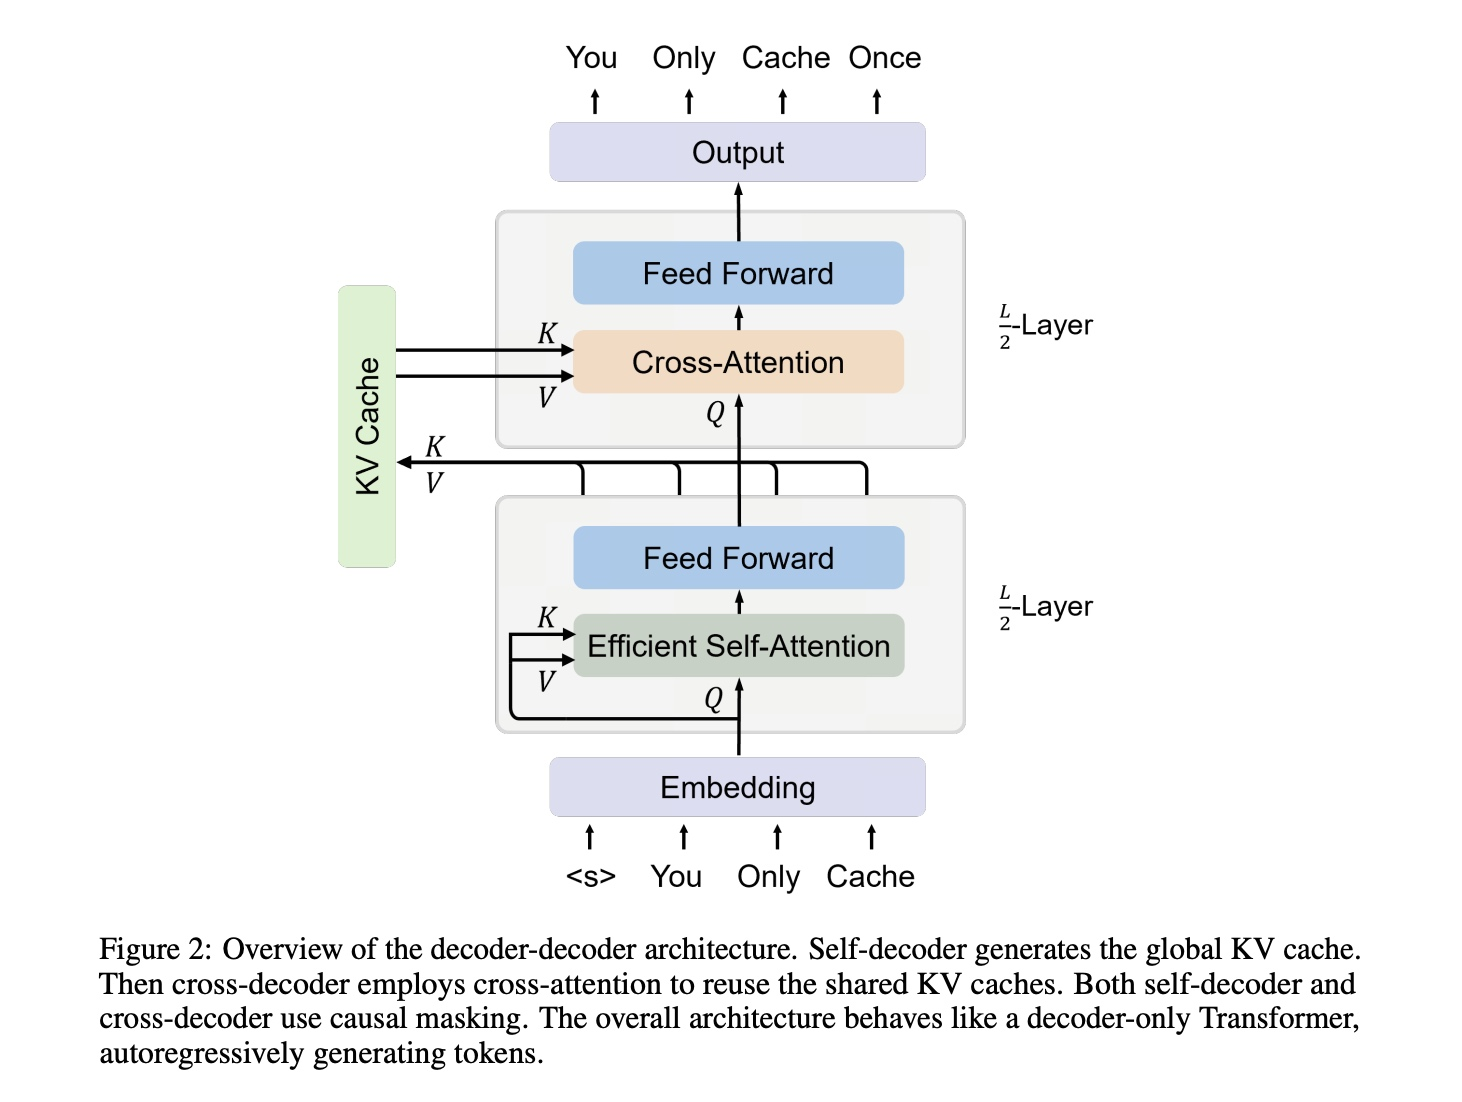
\includegraphics[width=0.7\linewidth,height=\textheight,keepaspectratio]{assets/YOCO_2.jpg}

\end{center}

\begin{center}

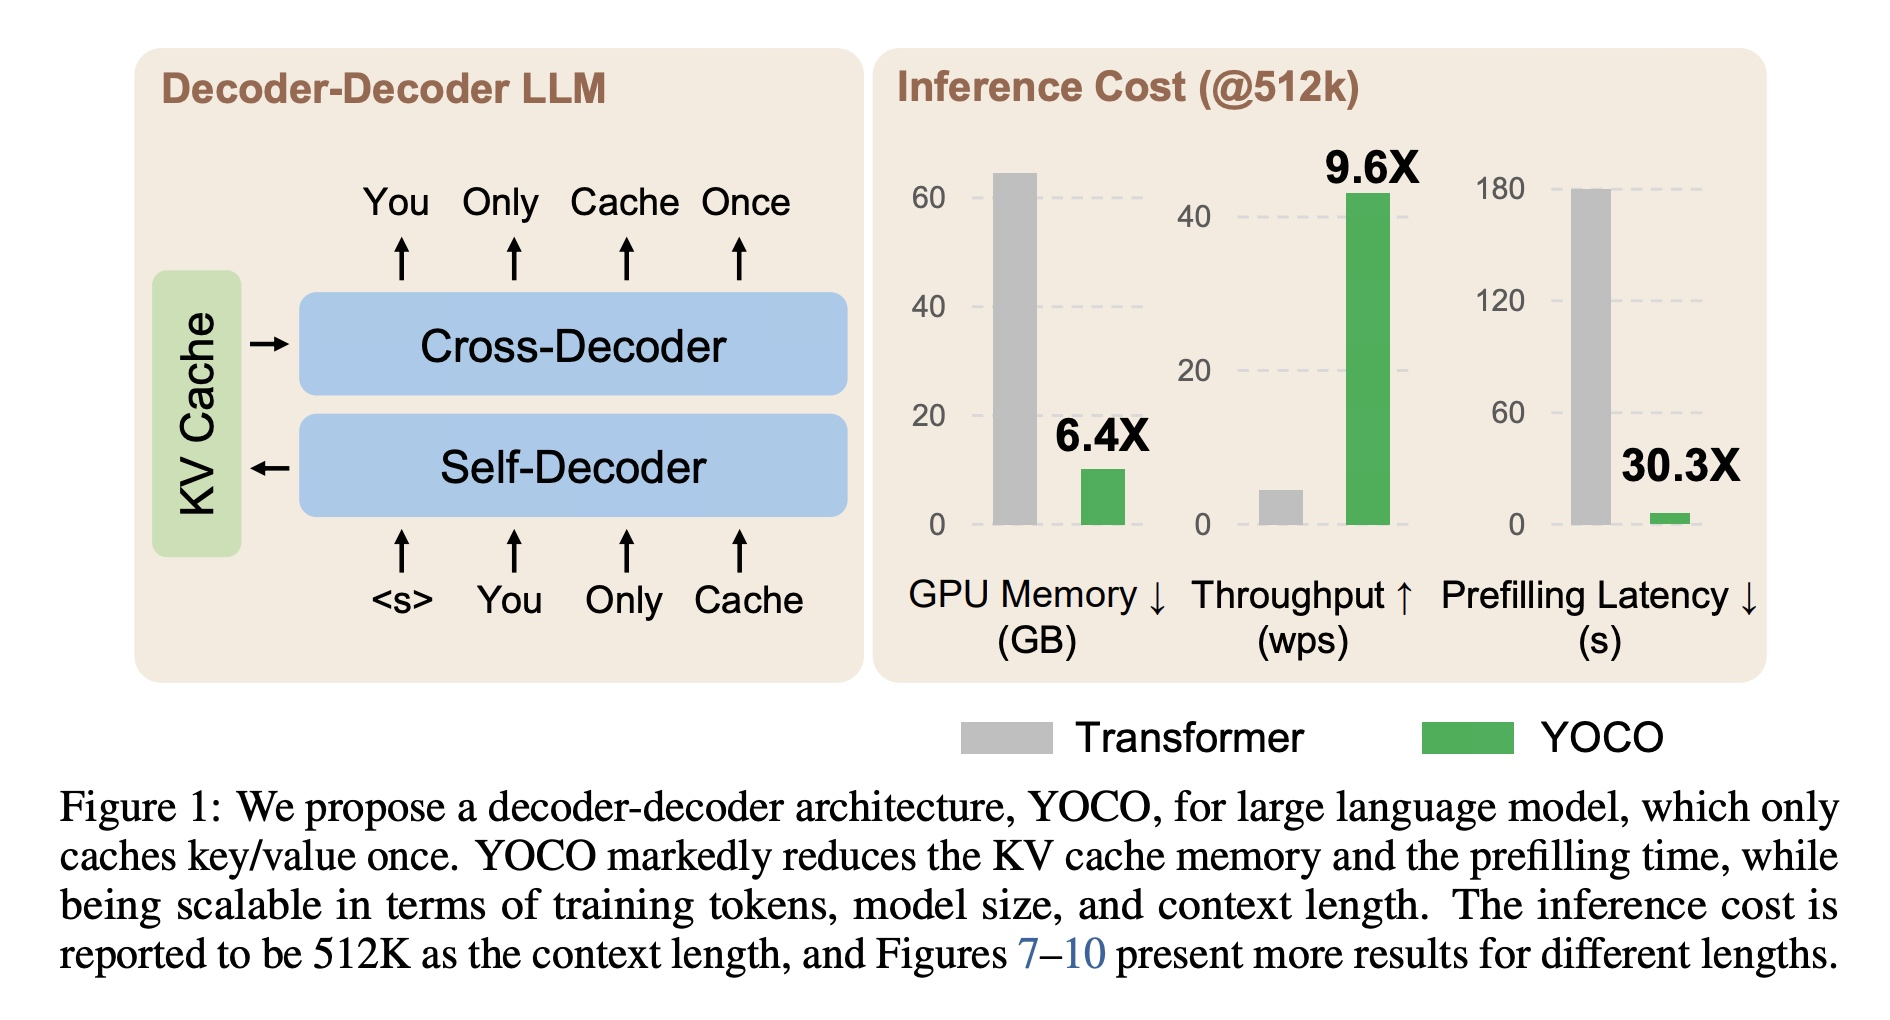
\includegraphics[width=0.9\linewidth,height=\textheight,keepaspectratio]{assets/YOCO_1.jpg}

\end{center}

YOCO's architecture is very straightforward: split a standard
decoder-only Transformer into two halves.

\textbf{The first half is the Self-Decoder.} More aggressively, this
part even uses gated retention or sliding-window attention to further
compress the entire context into \textbf{a shared global KV Cache}.

\textbf{The second half is the Cross-Decoder.} Each layer no longer
stores its own historical K/V. Instead, it uses its own Query to
cross-attend to the same shared KV.

The KV Cache cost of a standard Transformer drops from roughly
\(O(LND)\) to:

\[
O\!\left((N+L)D\right).
\]

Even better, Prefill does not need to run the later Cross-Decoder at all
(which is incredibly useful for the extremely long inputs in today's
agent scenarios).

\clearpage

\subsection{2. YOCO-U}\label{yoco-u}

\begin{center}

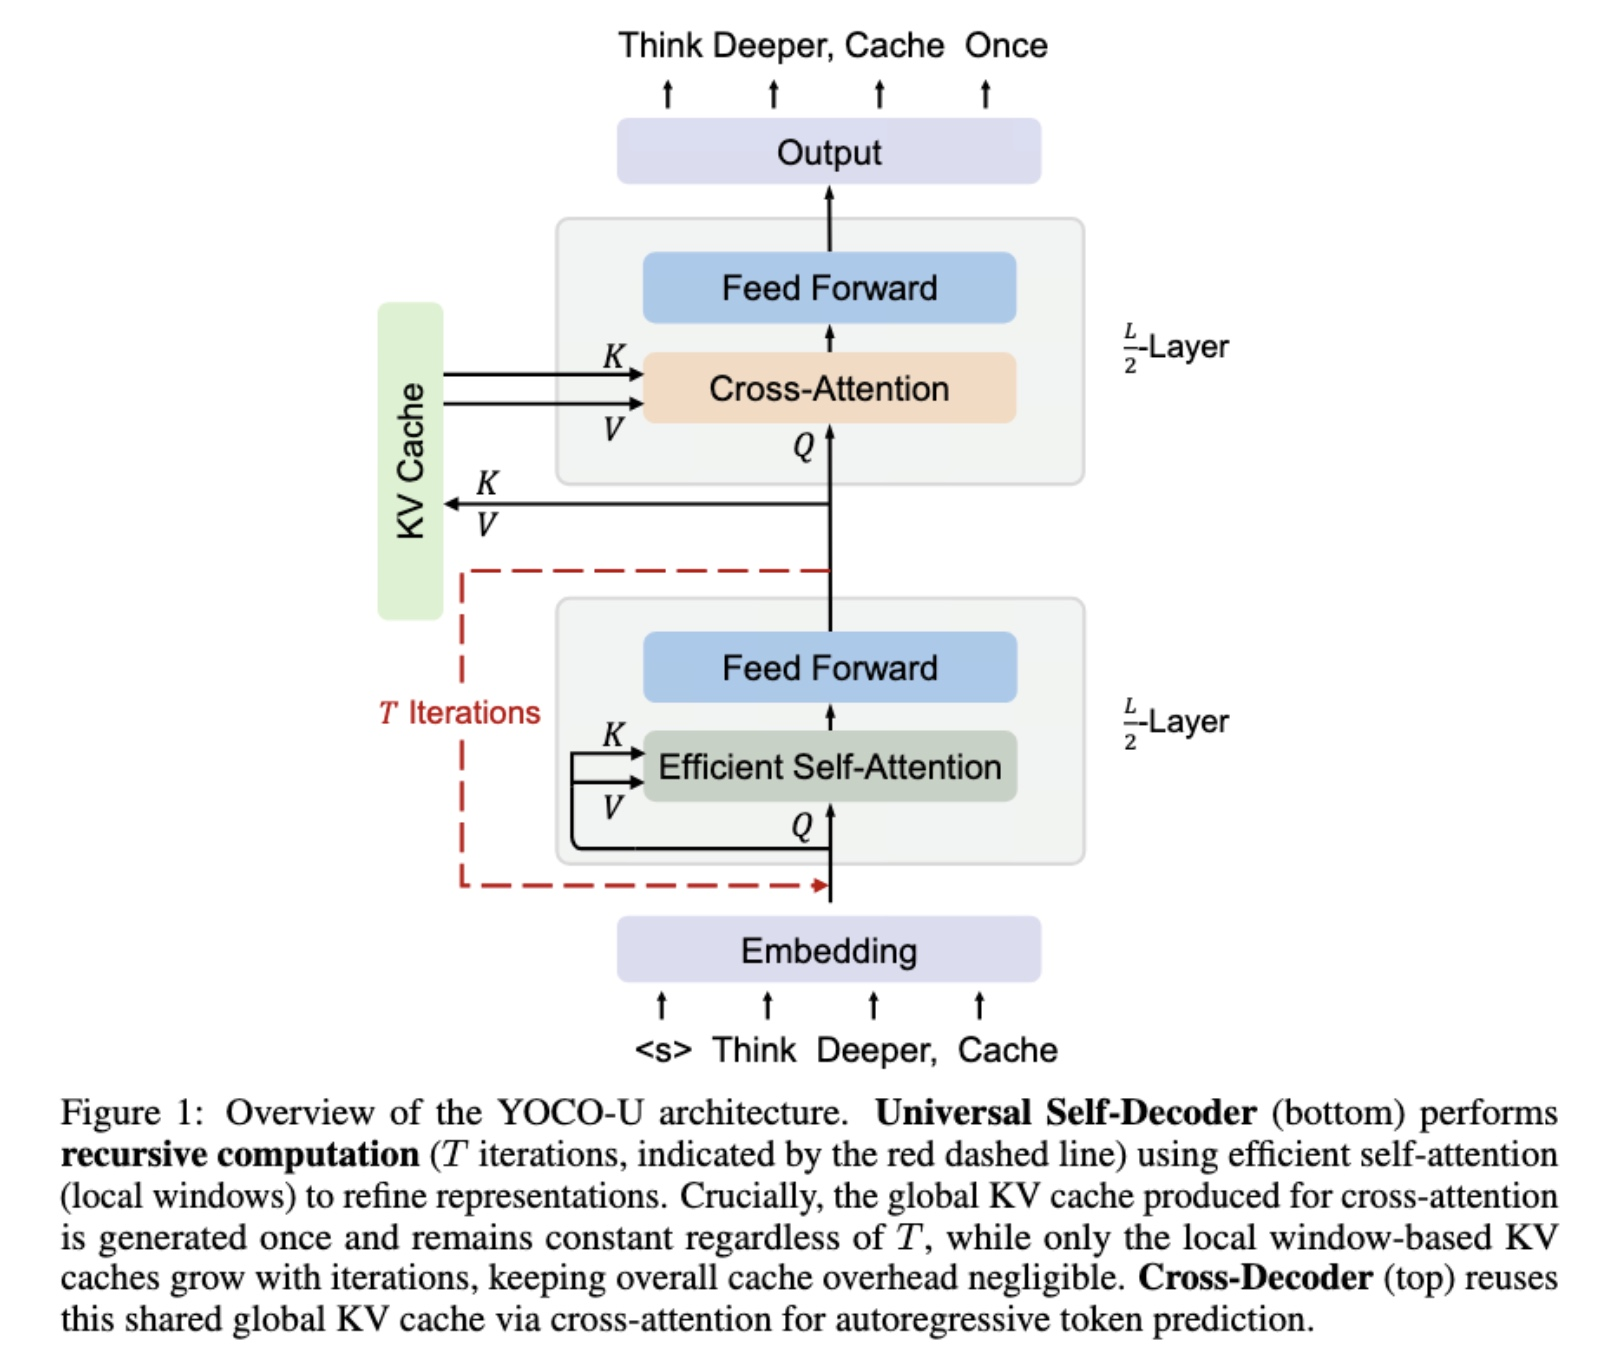
\includegraphics[width=0.65\linewidth,height=\textheight,keepaspectratio]{assets/YOCO-U_1.jpg}

\end{center}

YOCO-U adds \textbf{Loop} to the earlier Self-Decoder---that idea that
has remained shrouded in uncertainty while attracting wave after wave of
attention this year. It loops the Self-Decoder three times to produce a
Shared KV; the change on the Cross-Decoder side is to use \textbf{NOPE}.

\begin{center}

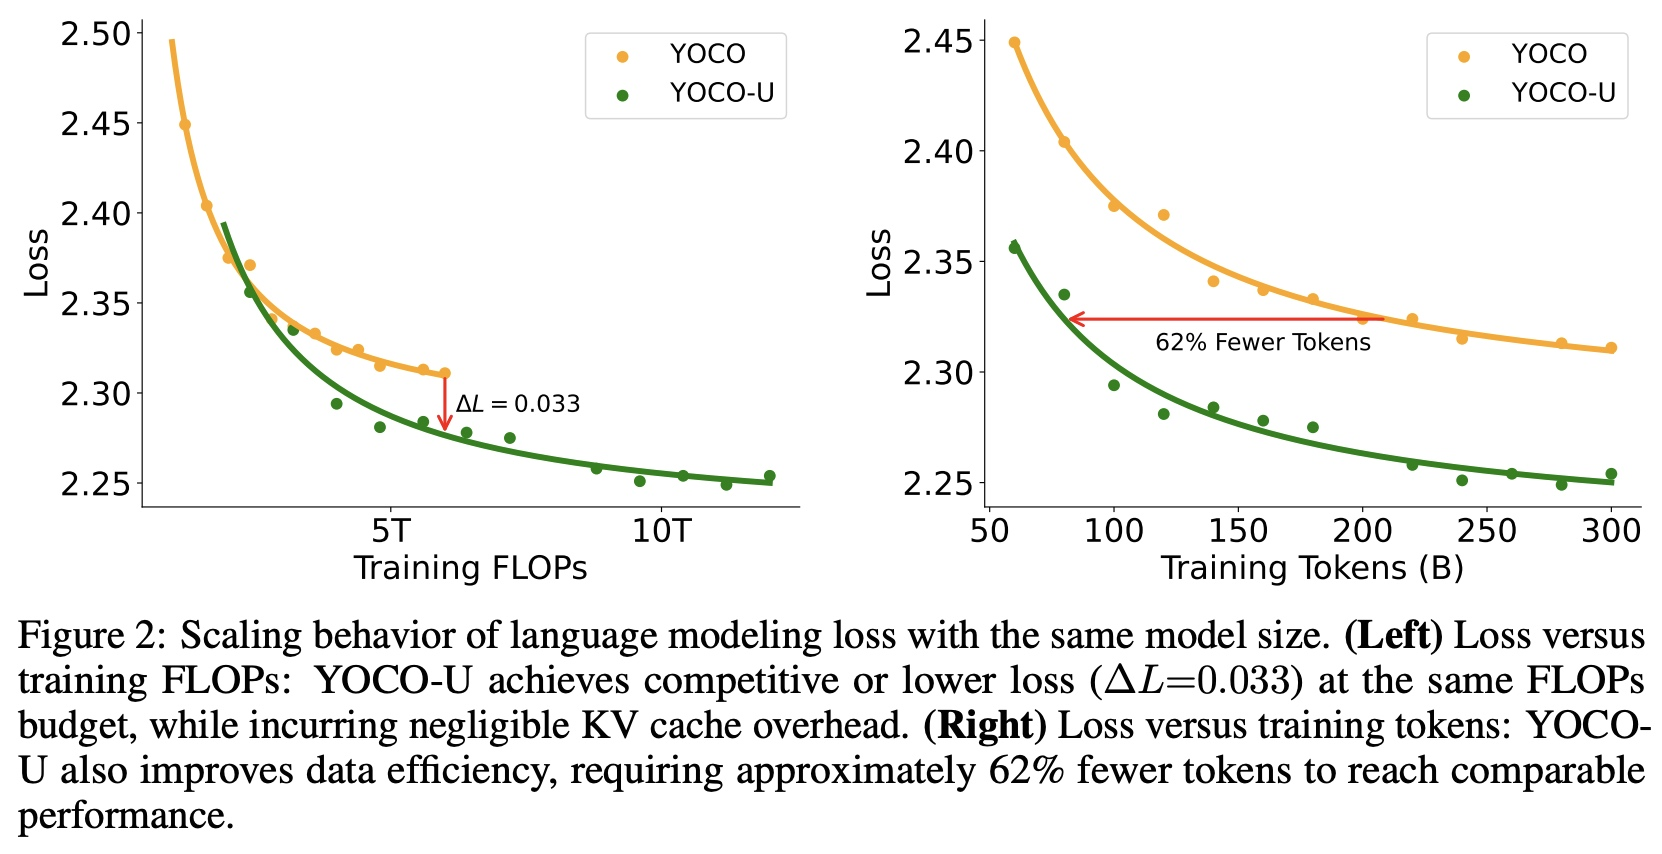
\includegraphics[width=0.75\linewidth,height=\textheight,keepaspectratio]{assets/YOCO-U_2.jpg}

\end{center}

\begin{center}

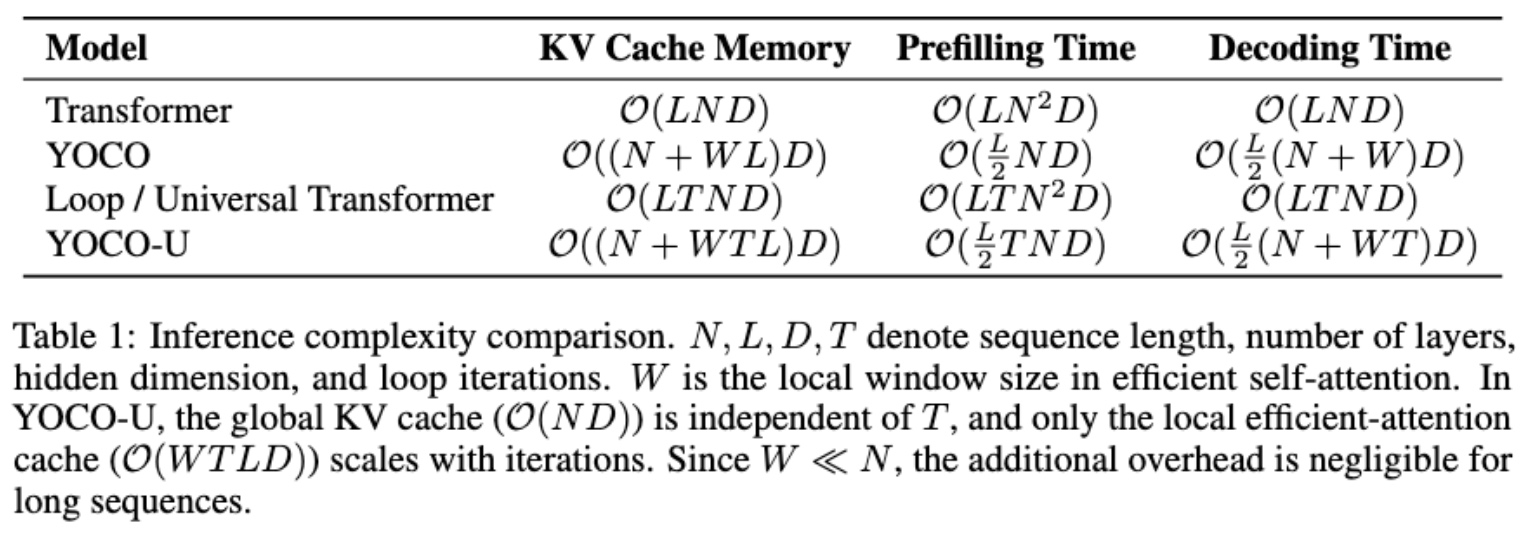
\includegraphics[width=0.8\linewidth,height=\textheight,keepaspectratio]{assets/YOCO-U_3.jpg}

\end{center}

\clearpage

\subsection{3. YOCO-Sparse}\label{yoco-sparse}

\begin{center}

\pandocbounded{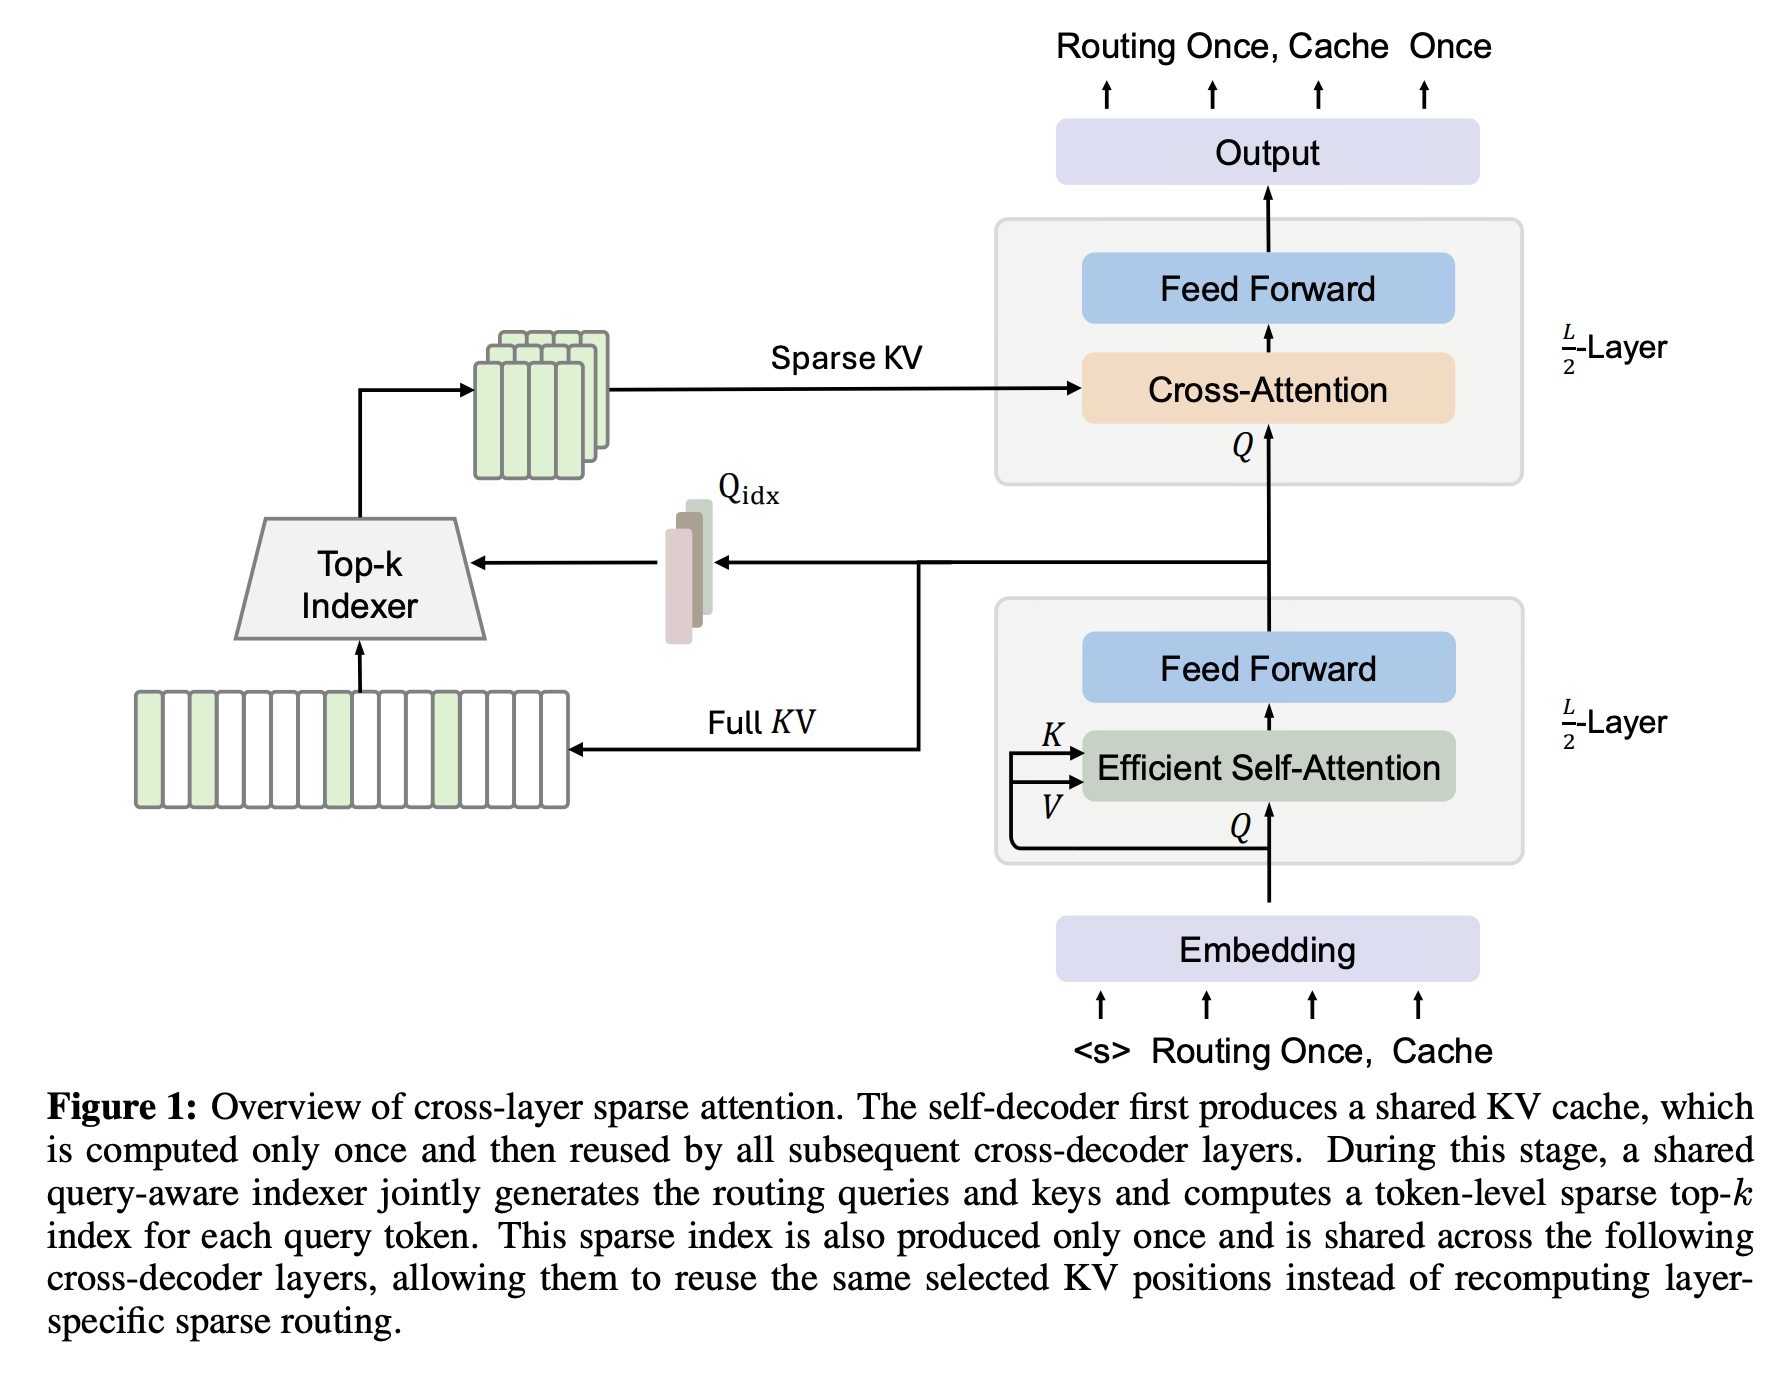
\includegraphics[keepaspectratio]{assets/YOCO-Sparse_1.jpg}}

\end{center}

YOCO-Sparse takes an even more direct approach: since multiple
Cross-Decoder layers in YOCO's second half already read the same KV
Cache, why not \textbf{share the Routing Index for Sparse Attention
too}? Savings on top of savings.

\begin{center}

\pandocbounded{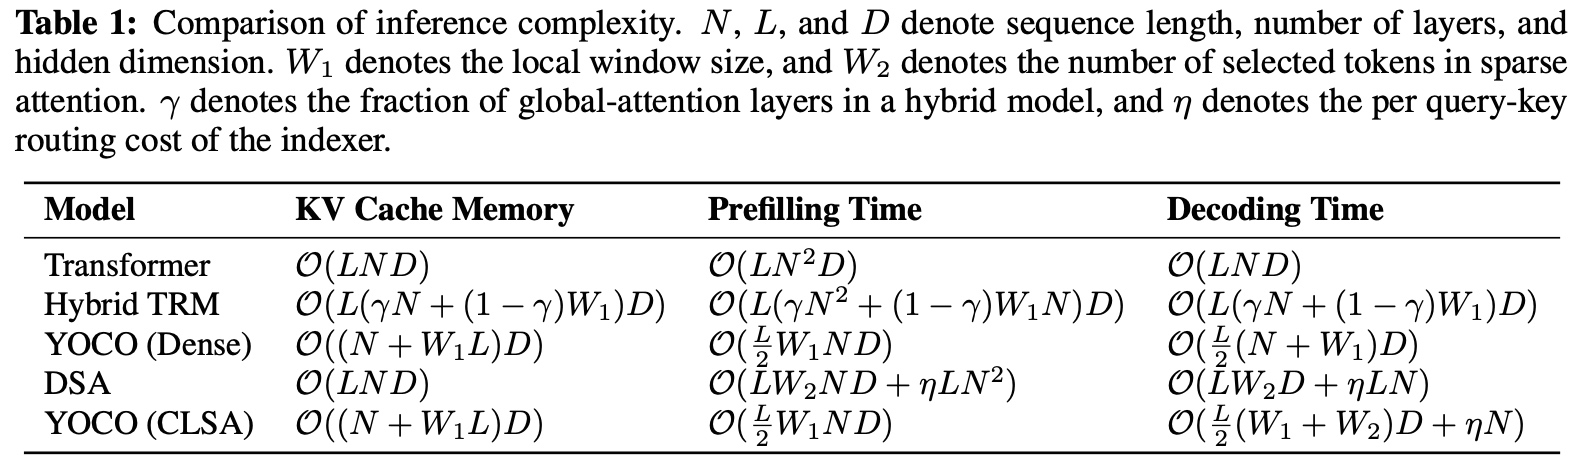
\includegraphics[keepaspectratio]{assets/YOCO-Sparse_2.jpg}}

\end{center}

\begin{center}

\pandocbounded{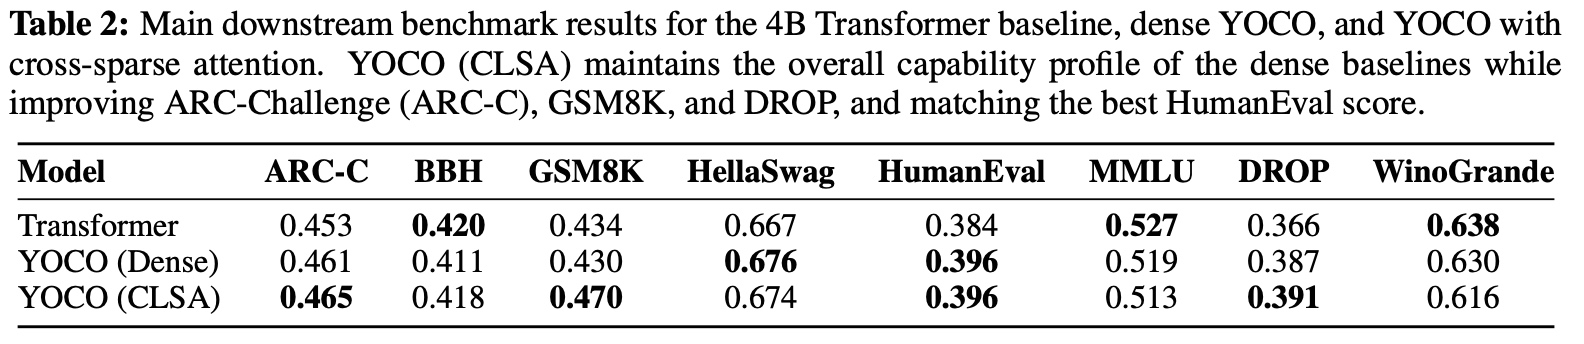
\includegraphics[keepaspectratio]{assets/YOCO-Sparse_3.jpg}}

\end{center}

\subsection{4. DeepSeek-V4.1-Flash}\label{deepseek-v4.1-flash}

\begin{center}

\pandocbounded{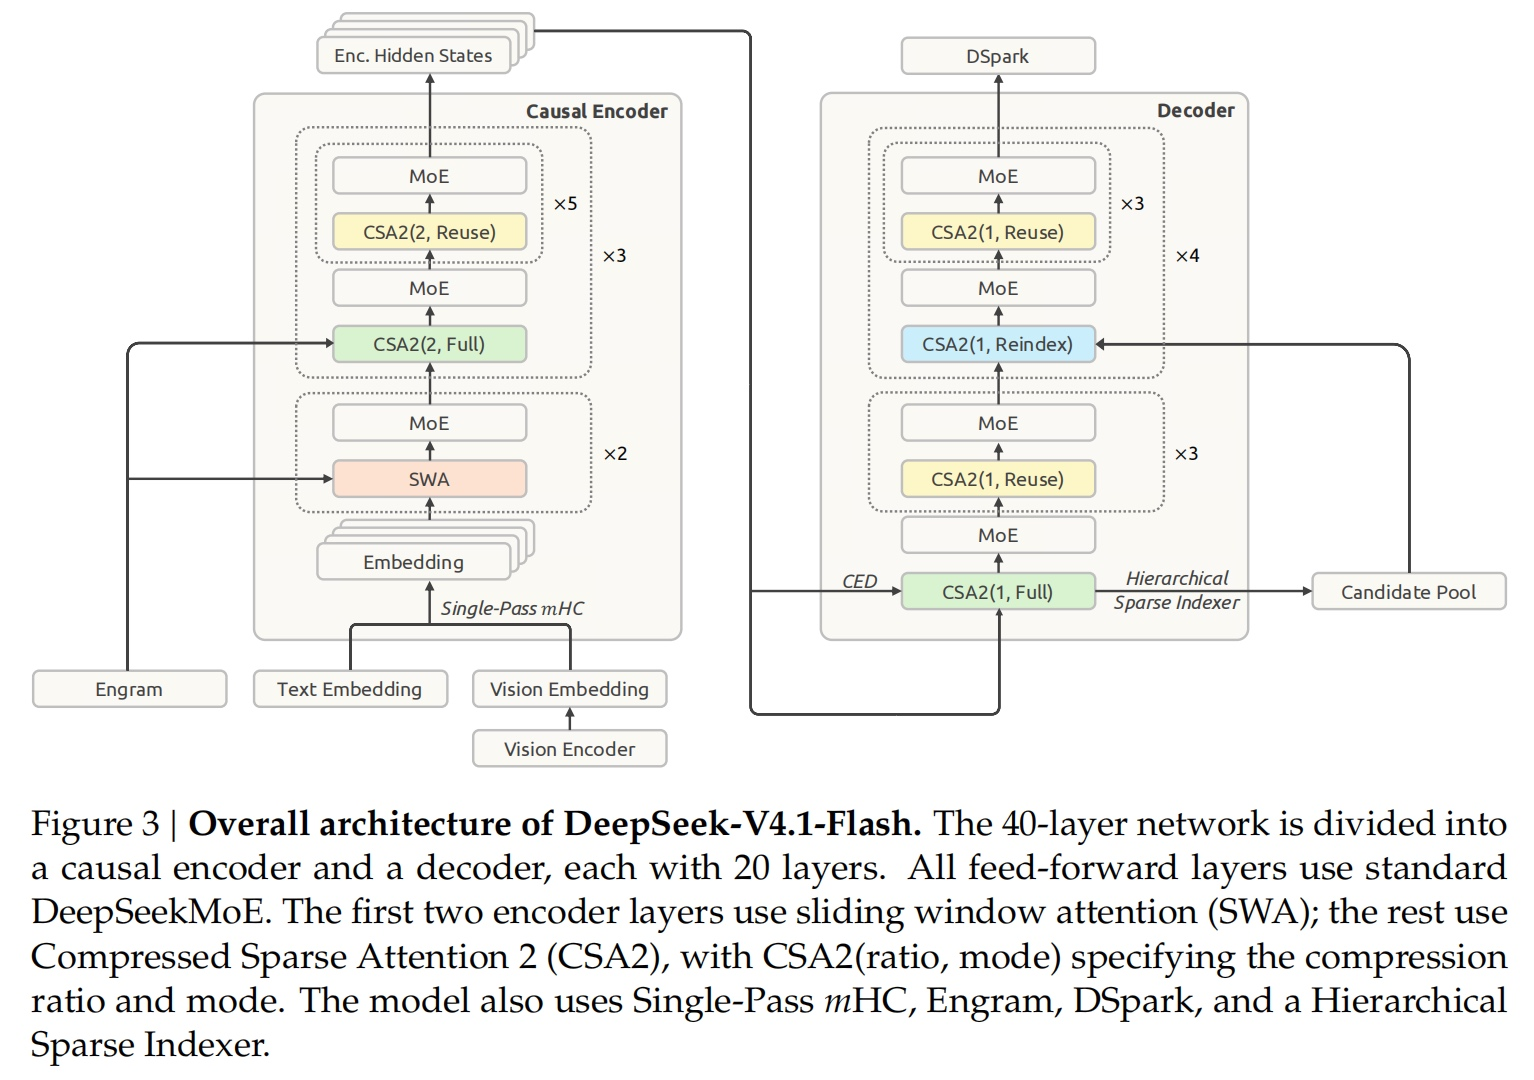
\includegraphics[keepaspectratio]{assets/DeepSeek-V4.1-Flash_1.jpg}}

\end{center}

DeepSeek has always been extremely, extremely, extremely aggressive
about compressing KV, and this time 4.1 takes it to a truly jaw-dropping
level.

\begin{center}

\pandocbounded{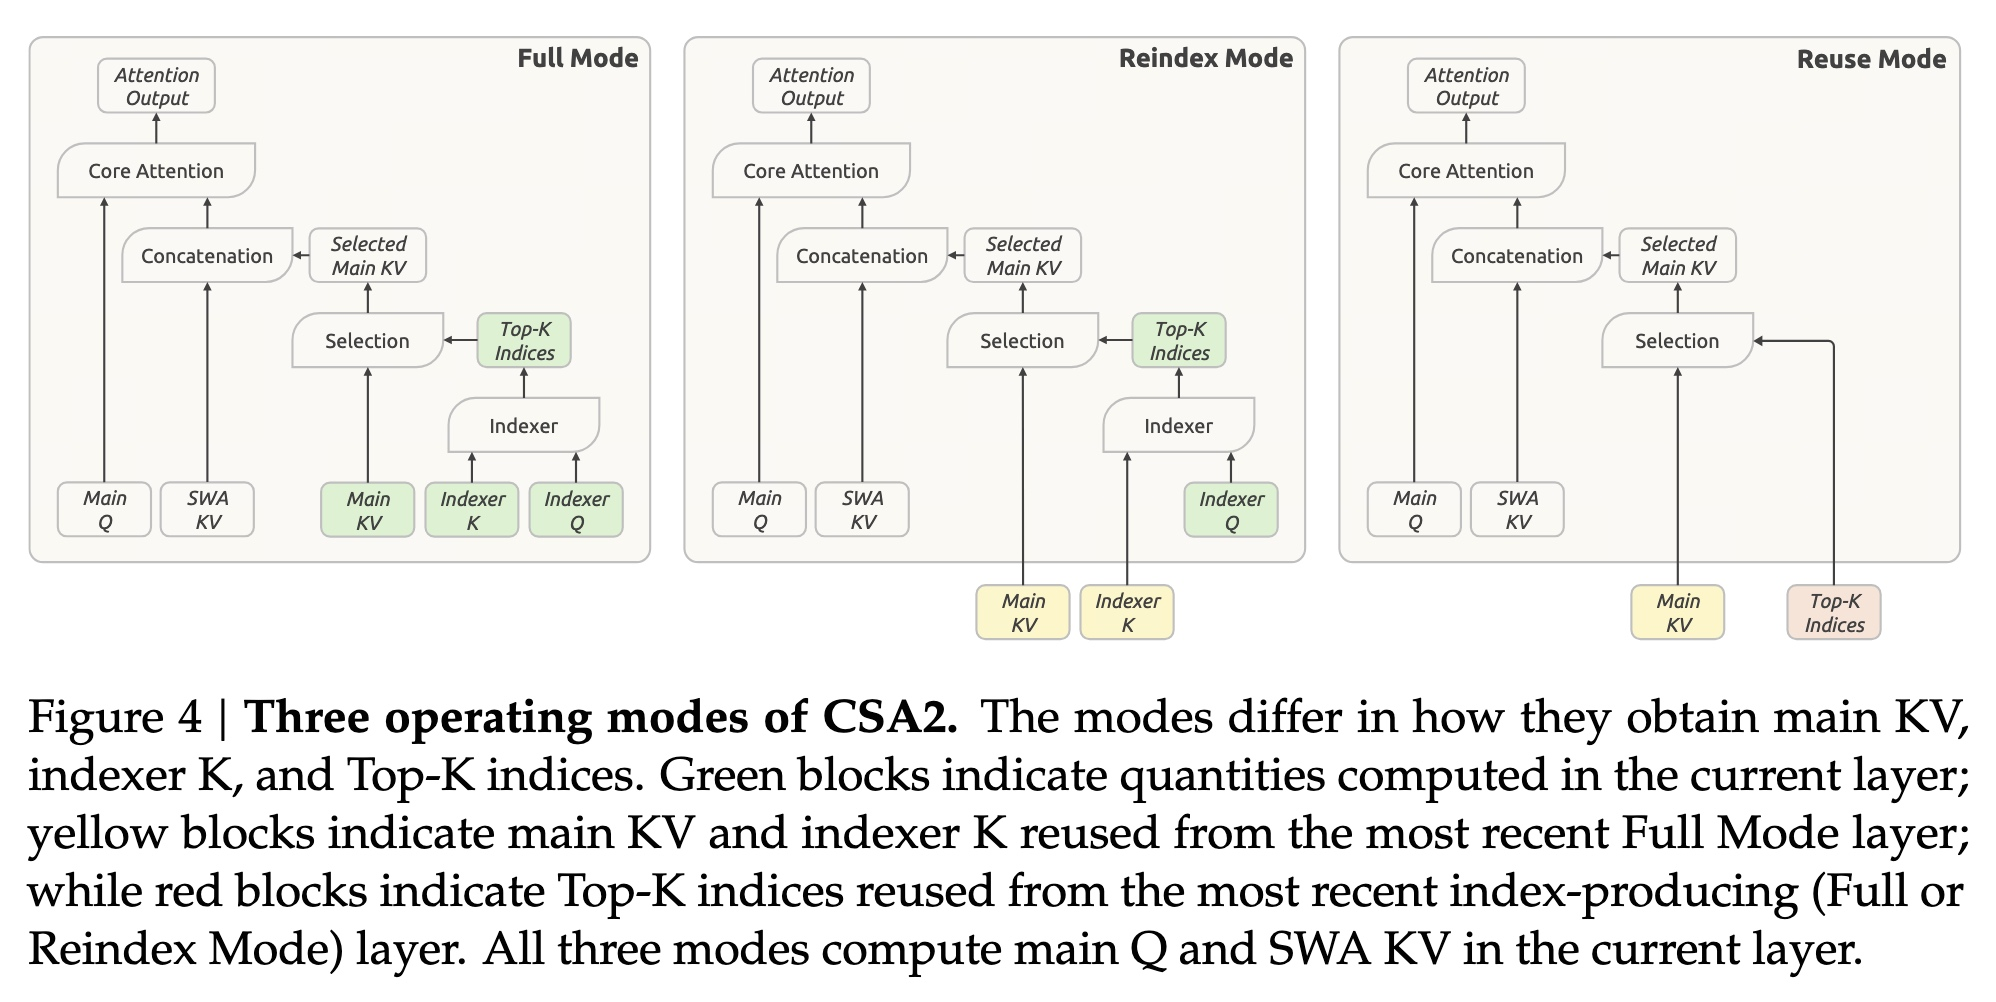
\includegraphics[keepaspectratio]{assets/DeepSeek-V4.1-Flash_2.jpg}}

\end{center}

DeepSeek-V4.1-Flash's Attention is roughly \textbf{YOCO/CED + CSA2 +
SWA}.

\subsubsection{YOCO/CED: Reducing Prefill
Computation}\label{yococed-reducing-prefill-computation}

Global KV follows the overall YOCO framework, splitting the 40 layers
into \textbf{a 20-layer Causal Encoder + a 20-layer Decoder}. DeepSeek
itself calls this the CED architecture.

During Prefill, the first 20 layers run. The Decoder's Global KV is
generated directly from the Encoder's final layer, \(H_{20}\), through
independent projections for each layer. This avoids running the entire
prompt through all of the last 20 layers again.

\subsubsection{CSA2: Reusing Global KV and Top-K Across
Layers}\label{csa2-reusing-global-kv-and-top-k-across-layers}

On top of this, Global Attention uses CSA2 for reuse across layers:

\begin{itemize}
\tightlist
\item
  \textbf{Full layers}: Generate new Global KV and Top-K.
\item
  \textbf{Reindex layers}: Reuse KV but select Top-K again.
\item
  \textbf{Reuse layers}: Reuse both KV and Top-K.
\end{itemize}

Within the Decoder, only the first Full layer generates Global KV.
Subsequent layers share this KV, with Reindex updating the retrieval
positions every few layers. Global Sparse Attention ultimately reads
only the \textbf{Top-512 remote KV entries}.

\subsubsection{SWA: Short-Term Caching and Local
Reconstruction}\label{swa-short-term-caching-and-local-reconstruction}

To save even more storage, DeepSeek no longer keeps SWA KV in the
persistent cache for the long term. What it mainly retains long-term is
Global KV, while SWA KV lives only in a host-DRAM pool with a short TTL.
\textbf{Global Main KV uses FP4, while SWA KV stays in FP8}.

If SWA KV is lost, reconstructing it would normally require replaying
\(128\times\text{layers}\) tokens, since the effective receptive field
of stacked SWA layers grows with the number of layers. But DS V4.1
simply \textbf{replays only the last 128 tokens} (it is so good at
squeezing out savings, I could cry\ldots).

During Decode, each new token still passes through all 40 layers as
usual, using \textbf{Top-512 Global Sparse KV + 128 Local SWA KV}
together.

\clearpage

\subsection{5. Gemma 4 E2B / E4B}\label{gemma-4-e2b-e4b}

Gemma 4 actually has quite a few architectural tricks, and E2B / E4B
also use a technique similar to YOCO.

The idea is simple and direct: \textbf{many layers in the later part
stop computing their own K/V, keep only their independent Q, and reuse
the KV from the last earlier Attention layer of the same type.}

{\def\LTcaptype{none} % do not increment counter
\begin{longtable}[]{@{}
  >{\raggedright\arraybackslash}p{(\linewidth - 8\tabcolsep) * \real{0.2000}}
  >{\raggedright\arraybackslash}p{(\linewidth - 8\tabcolsep) * \real{0.2000}}
  >{\raggedright\arraybackslash}p{(\linewidth - 8\tabcolsep) * \real{0.2000}}
  >{\raggedright\arraybackslash}p{(\linewidth - 8\tabcolsep) * \real{0.2000}}
  >{\raggedright\arraybackslash}p{(\linewidth - 8\tabcolsep) * \real{0.2000}}@{}}
\toprule\noalign{}
\begin{minipage}[b]{\linewidth}\raggedright
Model
\end{minipage} & \begin{minipage}[b]{\linewidth}\raggedright
Total Layers
\end{minipage} & \begin{minipage}[b]{\linewidth}\raggedright
Later Layers Sharing KV
\end{minipage} & \begin{minipage}[b]{\linewidth}\raggedright
Sliding Attention KV Source
\end{minipage} & \begin{minipage}[b]{\linewidth}\raggedright
Full / Global Attention KV Source
\end{minipage} \\
\midrule\noalign{}
\endhead
\bottomrule\noalign{}
\endlastfoot
\textbf{Gemma 4 E2B} & 35 & L15--L34 & KV from L13 & KV from L14 \\
\textbf{Gemma 4 E4B} & 42 & L24--L41 & KV from L22 & KV from L23 \\
\end{longtable}
}

\subsection{6. WeLM}\label{welm}

WeLM also does something similar to YOCO with \textbf{KV-Mirror}, but
its fundamental goal is not to save KV Cache; it is to \textbf{save
Prefill computation}.

Specifically, it uses \textbf{a U-shaped KV sharing strategy}: the first
third of the layers are mirrored to the last third for sharing. What is
reused is the mirrored layers' \textbf{Hidden States before the K/V
projections (not the KV!)}. The target layers' own projections then
recompute K/V, saving the full Attention, MoE, and other computations in
the last third of the layers during Prefill.

Why a U shape? An earlier paper, KVSharer, found that \textbf{sharing KV
between layers that differ more actually leads to better performance}.

\end{document}
